\begin{surferPage}[E6--]{An $E_6^{--}$ Singularity}
The following equation corresponds to the so-called $E_6^{--}$-singularity:
    \vspace*{-0.4em}
    \begin{center}
      $x^3-y^4-z^2=0.$
    \end{center}

  \vspace*{-0.7em}
    \begin{center}
      \begin{tabular}{c}
        \begin{tabular}{@{}c@{}}
          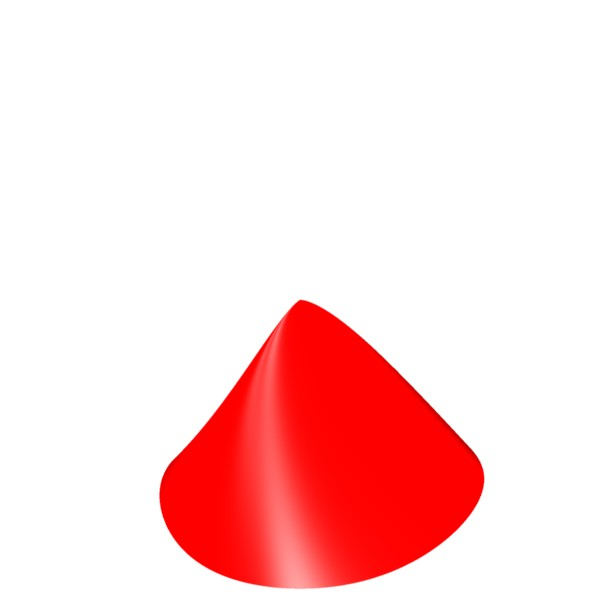
\includegraphics[width=1.2cm]{../../common/images/E6mm_0}
        \end{tabular}
        \end{tabular}
   \end{center}
    \vspace*{-0.4em}
 
It is not so easy to understand its geometry visually. 
 Two different ways are the following: 
deforming into two cusp singularities ($A_2$)
or into a $D_5$ singularity.
These can be seen by varying $a$ or $b$, respectively, 
in the following equation:
\[x^2\cdot ((0.5-b)x-by)-y^2\cdot(y-a)^2-z^2.\]

Keeping $b=0$ and varying $a$, we get:
    \begin{center}
      \begin{tabular}{@{}c@{\quad}c@{\quad}c@{}}
        \begin{tabular}{@{}c@{}}
          
\includegraphics[width=1.1cm]{../../common/images/E6mm_1}
        \end{tabular}
        &
        \begin{tabular}{@{}c@{}}
          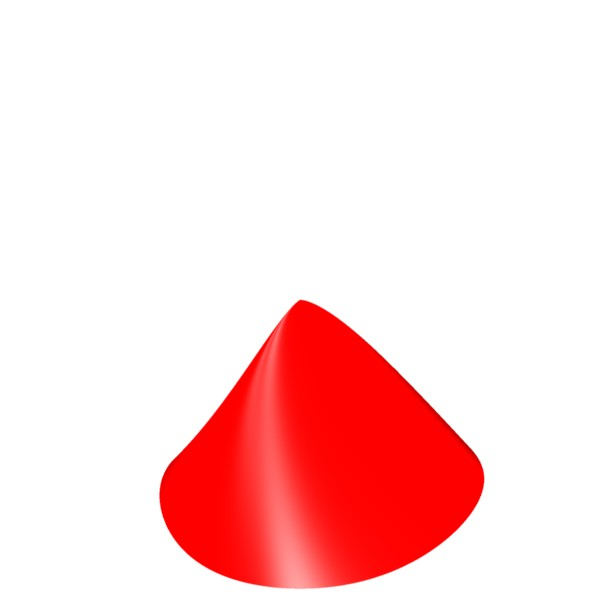
\includegraphics[width=1.1cm]{../../common/images/E6mm_0}
        \end{tabular}
        &
        \begin{tabular}{@{}c@{}}
          
\includegraphics[width=1.1cm]{../../common/images/E6mm_2}
        \end{tabular}
\\
$a=-0.5$
& 
$a=0$
&
$a=0.5$
      \end{tabular}
    \end{center}

On the other hand, keeping $a=0$ and varying $b$, we get:

   \begin{center}
      \begin{tabular}{@{}c@{\quad}c@{\quad}c@{}}
        \begin{tabular}{@{}c@{}}
          
\includegraphics[width=1.1cm]{../../common/images/E6mm_4}
        \end{tabular}
        &
        \begin{tabular}{@{}c@{}}
          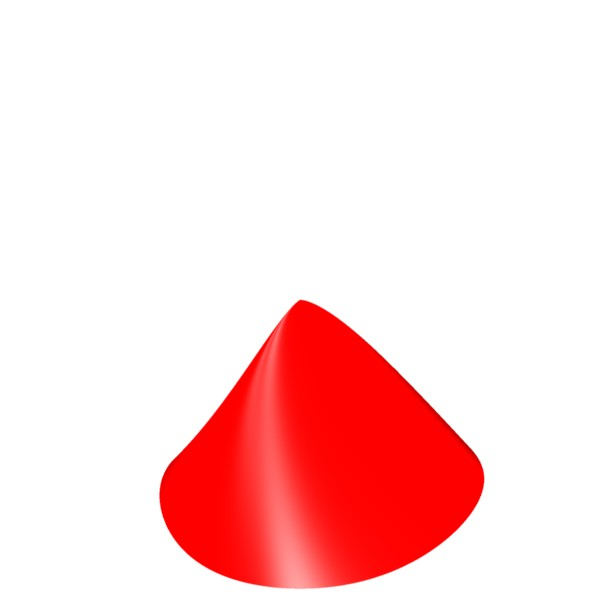
\includegraphics[width=1.1cm]{../../common/images/E6mm_0}
        \end{tabular}
        &
        \begin{tabular}{@{}c@{}}
          
\includegraphics[width=1.1cm]{../../common/images/E6mm_5}
        \end{tabular}
\\
$b=-0.5$
& 
$b=0$
&
$b=0.5$
      \end{tabular}
    \end{center}
 
\end{surferPage}
